% document type
\documentclass[12pt]{article}

% packages
\usepackage[total={170mm,230mm}]{geometry}
\usepackage[utf8]{inputenc}
\usepackage[T1]{fontenc}
\usepackage[russian]{babel}
\usepackage{graphicx}
\usepackage{amssymb}
\usepackage{amsfonts}
\usepackage{amsmath}
\usepackage{amsthm}
\usepackage{physics}
\usepackage{nicefrac}
\usepackage{cancel}
\usepackage[unicode, colorlinks=true]{hyperref}
\usepackage{cmap}
\usepackage{multirow}
\usepackage{tabularx}
\usepackage{extarrows}
\usepackage{physics}
\usepackage{amsmath}
\usepackage{tikz}
\usepackage{mathdots}
\usepackage{yhmath}
\usepackage{cancel}
\usepackage{color}
\usepackage{siunitx}
\usepackage{array}
\usepackage{multirow}
\usepackage{amssymb}
\usepackage{gensymb}
\usepackage{tabularx}
\usepackage{extarrows}
\usepackage{booktabs}
\usetikzlibrary{fadings}
\usetikzlibrary{patterns}
\usetikzlibrary{shadows.blur}
\usetikzlibrary{shapes}

\title{Лабораторная работа №1}
\author{Александр Козлов\and Алексей Чубаров}
\date{}
\begin{document}
\maketitle

\section{Кольца Ньютона}
\subsection{Определение масштабного коэффициента}
Для определения масштабный коэффициент определим сколько пикселей в одном миллиметре. Будем работать со шкалой, представленной на рисунке \ref{fig:1}. 
\begin{figure}[htbp]
	\centering
	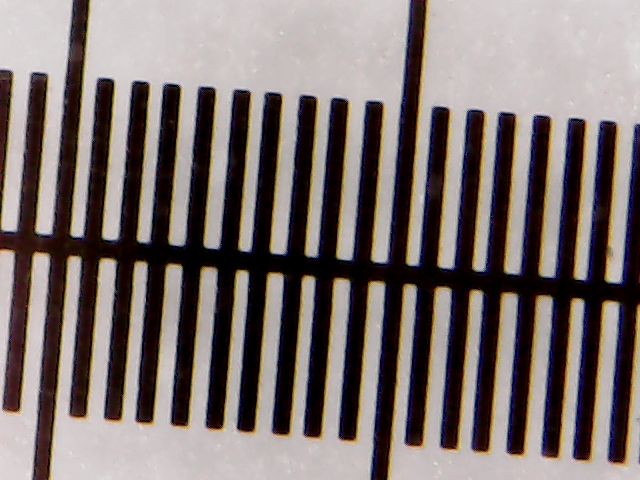
\includegraphics[width = 0.5\linewidth]{data/1-0.jpg}
	\caption{Нониусная шкала колибратора. Между двумя соседними маленькими отметками лежит одна десятая часть миллиметра. Ось шкалы находится под углом $5^\circ$ к горизонту.}
	\label{fig:1}
\end{figure}
В 12 сверху строке пикселей имеется картина интенсивностей, изображённая на рисунке \ref{fig:2}, откуда можно определить расстояние между двумя большими чёрными праллельными полосами.
\begin{figure}[htbp]
	\centering
	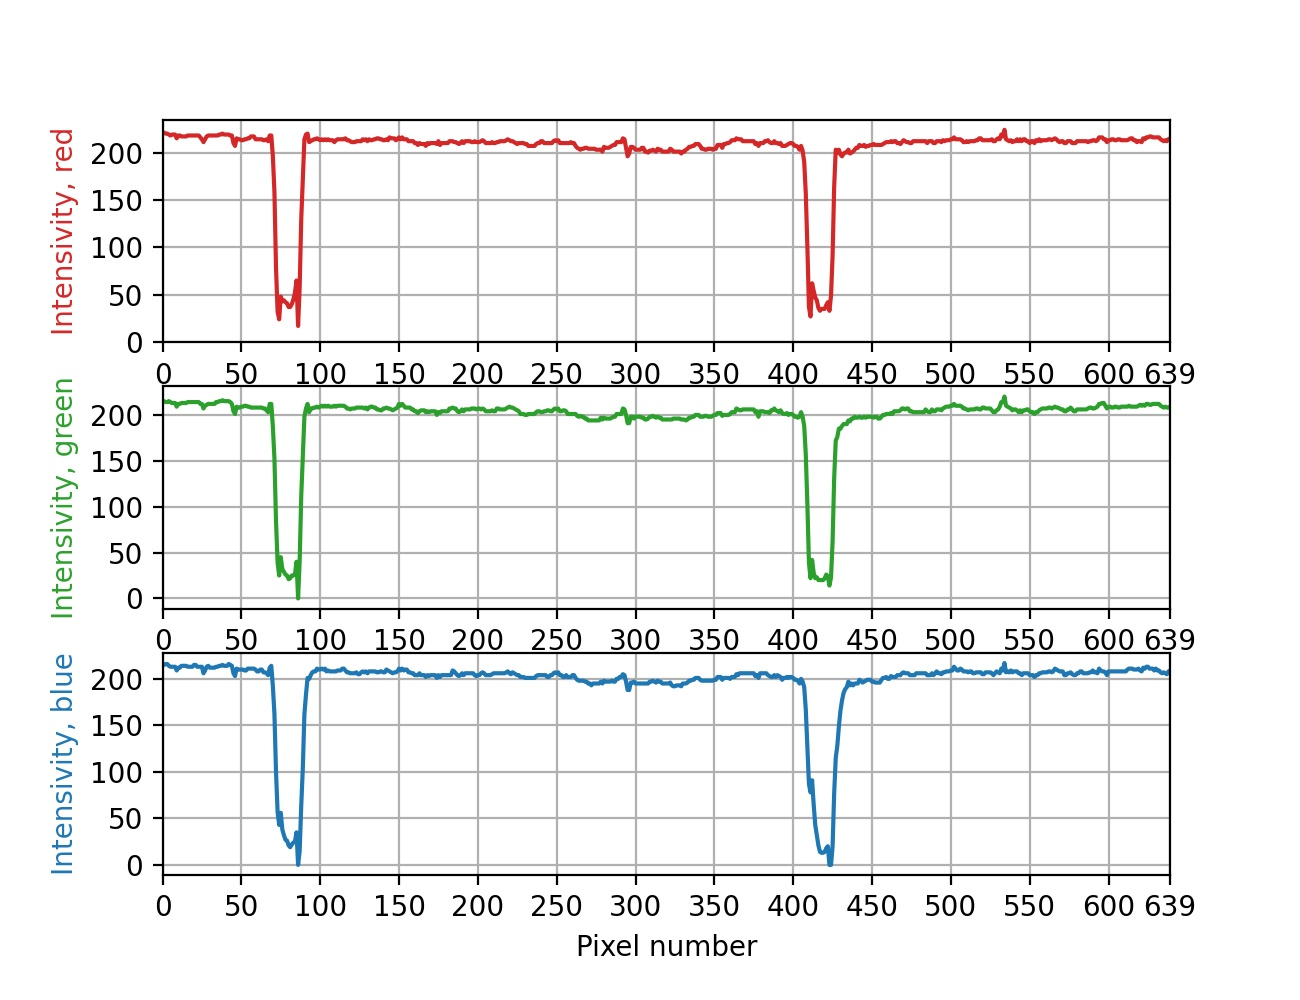
\includegraphics[scale = 1]{plots/1-0.jpg}
	\caption{Интенсивность пикселей в 12 строке сверху изображения \ref{fig:1}.}
	\label{fig:2}
\end{figure}
Результаты таких измерений занесены в таблицу \ref{tab:1}. Точность определения положений примем равной $10$ пикселям (так как ширина углублений на графиках интенсивностей составляется пимерно $20$ пикселей). Тогда точность определения расстояний составит $20$ пикселей. Усреднённое по цветам расстояние между длинными черными полосами будет равно $338\pm20$ пикселей. 
\par Но стоит так же учесть наклон оси шкалы к горизонту (тут под горизонтом понимается горизонтальная ось), который составляет $5^\circ\pm0.25^\circ$. Из элементарных геометрических соображений ясно, что нужно умножить определённое ранее расстояние на косинус угла наклона. Тогда получим, что правильное расстояние между двумя длинными полосами составляет $333\pm20$ пикселей. 
\begin{table}
\centering
\caption{\label{tab:1}Результаты измерений расстояний между черными длинными полосами для различных цветов.}
\begin{tabular}{|l|l|l|l|} 
\hline
Цвет    & \begin{tabular}[c]{@{}l@{}}Положение\\левой полосы,\\пиксели\end{tabular} & \begin{tabular}[c]{@{}l@{}}Положение\\правой полосы,\\пиксели\end{tabular} & \begin{tabular}[c]{@{}l@{}}Расстояние между\\двумя черными полосами, \\пиксели\end{tabular}  \\ 
\hline
Красный & 80                                                                        & 416                                                                        & 336                                                                                          \\ 
\hline
Зелёный & 80                                                                        & 417                                                                        & 337                                                                                          \\ 
\hline
Синий   & 80                                                                        & 420                                                                        & 340                                                                                          \\
\hline
\end{tabular}
\end{table}
Здесь для вычисления погрешности использовалась формула
\begin{equation}
	\dd l_{new} = \dd \qty(l_{old}\cdot\cos{\theta}) = \dd l_{old} \cdot \cos{\theta} + l_{old} \cdot \sin{\theta} \cdot \dd \theta,
\end{equation}
где угол $\theta$ выражен в радианах. Таким образом, $1$ мм соответствует $333\pm20$ пикселей, значит, масштабный коэффициент будет равен
\begin{equation}
	k = 3 \dfrac{\text{мкм}}{\text{пиксель}}.
\end{equation}
Погрешность будет равна примерно $0$, ибо согласно формуле для погрешности
\begin{equation}
	\dd \dfrac1l = \dfrac{\dd l}{l^2} = 0.12\ {\text{пиксель}}^{-1}
\end{equation}
она получается мала и при окгруглении до значящих порядков становится равной нулю.

\subsection{Вычисление радиуса кривизны.}
Для начала найдём с учётом масштабного коэффициента значения квадратов радиуса и построим линейную аппроксимацию (см. рис~\ref{fig:3}). Затем вычислим погрешности для угловых коэффициентов в наших зависимостях. Запишем результаты данных вычислений в таблицу.
\begin{figure}[htbp]
	\centering
	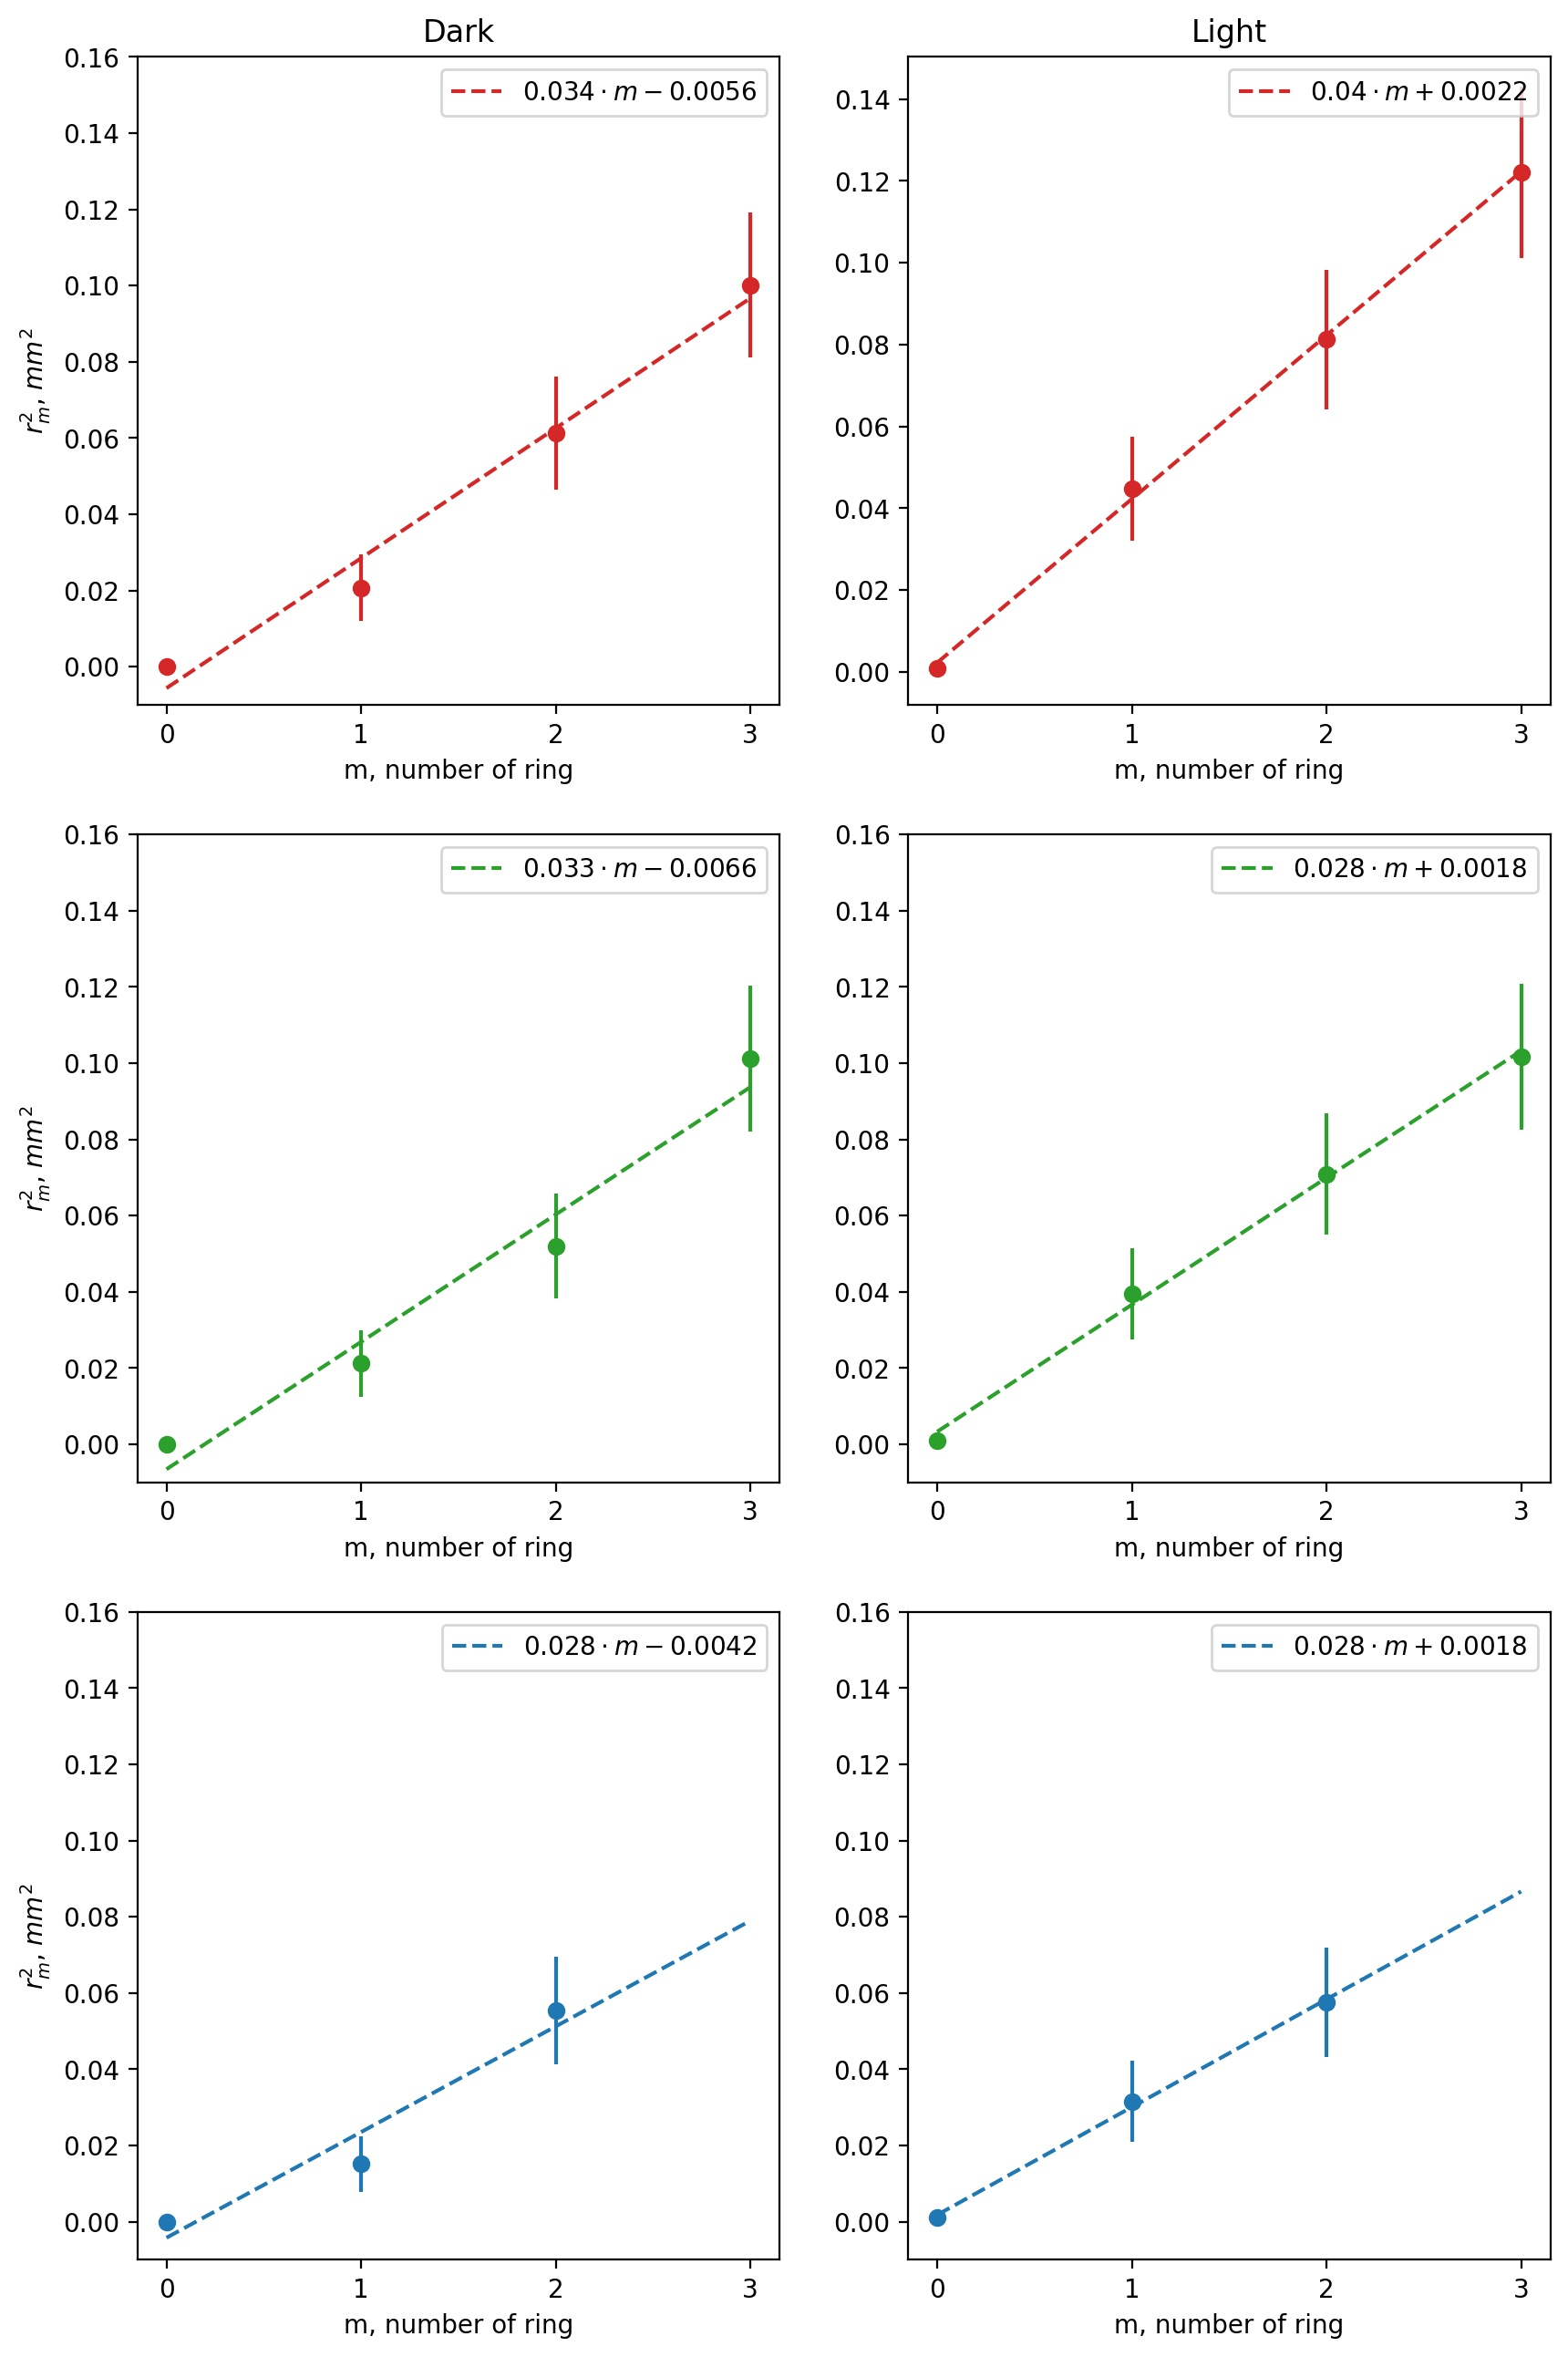
\includegraphics[scale = 0.65]{plots/1-1.jpg}
	\caption{Графики зависимостей $r_m^2(m)$ для разных цветов.}
	\label{fig:3}
\end{figure}





			
	\begin{tabular}{|p{0.13\textwidth}|p{0.13\textwidth}|p{0.16\textwidth}|p{0.16\textwidth}|p{0.20\textwidth}|}
		\hline 
		\begin{center}
			цвет
		\end{center}
		& \begin{center}
			тип полос
		\end{center}
		& \begin{center}
			значение углового коэффициента
		\end{center}
		& \begin{center}
			абсолютная погрешность
		\end{center}
		& \begin{center}
			относительная погрешность
		\end{center}
		\\
		\hline 
		\begin{center}\multirow{2}{*}{
				красный
			}\end{center} & \begin{center}
			тёмный
		\end{center}
		& \begin{center}
			$\displaystyle 0,034$
		\end{center}
		& \begin{center}
			$\displaystyle 0,003$
		\end{center}
		& \begin{center}
			$\displaystyle 0,09$
		\end{center}\\
		\cline{2-5} 
		& \begin{center}
			светлый
		\end{center}
		& \begin{center}
			$\displaystyle 0,040$
		\end{center}
		& \begin{center}
			$\displaystyle 0,001$
		\end{center}
		& \begin{center}
			$\displaystyle 0,025$
		\end{center}
		\\ 
		\hline 
		\begin{center}\multirow{2}{*}{зелёный}\end{center} & \begin{center}
			тёмный
		\end{center}
		& \begin{center}
			$\displaystyle 0,033$
		\end{center}
		& \begin{center}
			$\displaystyle 0,004$
		\end{center}
		& \begin{center}
			$\displaystyle 0,12$
		\end{center}
		\\
		\cline{2-5} 
		& \begin{center}
			светлый
		\end{center}
		& \begin{center}
			$\displaystyle 0,028$
		\end{center}
		& \begin{center}
			$\displaystyle 0,001$
		\end{center}
		& \begin{center}
			$\displaystyle 0,04$
		\end{center}
		\\
		\hline 
		\begin{center}\multirow{2}{*}{синий
			}\end{center} & \begin{center}
			тёмный
		\end{center}
		& \begin{center}
			$\displaystyle 0,028$
		\end{center}
		& \begin{center}
			$\displaystyle 0,007$
		\end{center}
		& \begin{center}
			$\displaystyle 0,25$
		\end{center}
		\\
		\cline{2-5} 
		& \begin{center}
			светлый
		\end{center}
		& \begin{center}
			$\displaystyle 0,028$
		\end{center}
		& \begin{center}
			$\displaystyle 0,001$
		\end{center}
		& \begin{center}
			$\displaystyle 0,04$
		\end{center}
		\\
		\hline
	\end{tabular}
	
	Теперь вычислим по этим данным радиус кривизны воспользовавшись тем, что 
	\begin{equation*}
		\text{``угловой коэффициент''}=2\cdot R\cdot \lambda,
	\end{equation*}
	где $R$ --- радиус кривизны, который нам и нужно найти, а $\lambda$ --- длина волны света. Воспользовавшись этой формулой получим следующее
	
	
		\begin{tabular}{|p{0.20\textwidth}|p{0.13\textwidth}|p{0.13\textwidth}|p{0.15\textwidth}|p{0.16\textwidth}|}
			\hline 
			\begin{center}
				цвет
			\end{center}
			& \begin{center}
				тип полос
			\end{center}
			& \begin{center}
				$\displaystyle R,$ мм
			\end{center}
			& \begin{center}
				абсолютная погрешность
			\end{center}
			& \begin{center}
				относительная погрешность
			\end{center}
			\\
			\hline 
			\begin{center}\multirow{2}{*}{
					красный ($\displaystyle 600$ нм)
				}\end{center} & \begin{center}
				тёмный
			\end{center}
			& \begin{center}
				$\displaystyle 28$
			\end{center}
			& \begin{center}
				$\displaystyle 3$
			\end{center}
			& \begin{center}
				$\displaystyle 0,09$
			\end{center}
			\\
			\cline{2-5} 
			& \begin{center}
				светлый
			\end{center}
			& \begin{center}
				$\displaystyle 33,3$
			\end{center}
			& \begin{center}
				$\displaystyle 0,8$
			\end{center}
			& \begin{center}
				$\displaystyle 0,025$
			\end{center}
			\\
			\hline 
			\begin{center}\multirow{2}{*}{
					зелёный ($\displaystyle 550$ нм) 
			}\end{center} & \begin{center}
				тёмный
			\end{center}
			& \begin{center}
				$\displaystyle 30$
			\end{center}
			& \begin{center}
				$\displaystyle 4$
			\end{center}
			& \begin{center}
				$\displaystyle 0,12$
			\end{center}
			\\
			\cline{2-5} 
			& \begin{center}
				светлый
			\end{center}
			& \begin{center}
				$\displaystyle 25$
			\end{center}
			& \begin{center}
				$\displaystyle 1$
			\end{center}
			& \begin{center}
				$\displaystyle 0,04$
			\end{center}
			\\
			\hline 
			\begin{center}\multirow[b]{2}{*}{
					синий ($\displaystyle 460$ нм) 			}\end{center} & \begin{center}
				тёмный
			\end{center}
			& \begin{center}
				$\displaystyle 30$
			\end{center}
			& \begin{center}
				$\displaystyle 8$
			\end{center}
			& \begin{center}
				$\displaystyle 0,25$
			\end{center}
			\\
			\cline{2-5} 
			& \begin{center}
				светлый
			\end{center}
			& \begin{center}
				$\displaystyle 30$
			\end{center}
			& \begin{center}
				$\displaystyle 1$
			\end{center}
			& \begin{center}
				$\displaystyle 0,04$
			\end{center}
			\\
			\hline
		\end{tabular}
		\vspace{0.2cm}
		
	Таким образом радиус кривизны линзы составляет примерно $30$ мм.
	
	 
\end{document}